\chapter{AI Techniques and Dashboard Implementation}
\label{ch:techimpl}

This chapter provides the complete engineering specification of two core technical
components of this project: the Artificial Intelligence (AI) techniques pipeline and
the interactive compliance dashboard. Together with the RAG module documented in
Chapter~\ref{ch:rag}, these components form an integrated system that transforms
curated regulatory data into an explorable, evidence-grounded analytics platform.

Section~\ref{sec:full-pipeline} presents the complete system architecture connecting
all four pipeline stages. Section~\ref{sec:ai-full} covers AI techniques in depth.
Section~\ref{sec:dash-full} documents the interactive dashboard implementation.
Section~\ref{sec:integration} closes with system integration and validation.

% -------------------------------------------------------------------------------
\section{Methodological Pipeline: Complete Architecture}
\label{sec:full-pipeline}
% -------------------------------------------------------------------------------

\subsection{Design Philosophy}
\label{sec:pipeline-philosophy}

The system is built on three interlocking principles derived from the project
objectives and from responsible-AI engineering practice:

\begin{enumerate}[noitemsep]
  \item \textbf{Retrieve before generating} --- no claim is output unless it is
        grounded in an indexed passage with a traceable citation;
  \item \textbf{Human in the loop} --- the AI pipeline accelerates evidence
        scanning but humans retain authority over score assignments and public
        claims;
  \item \textbf{Reproducibility by design} --- all data, code, and configuration
        are version-controlled so that any examiner can regenerate the report.
\end{enumerate}

These principles directly shape every implementation choice that follows.

\subsection{Full System Architecture}
\label{sec:full-arch}

Figure~\ref{fig:full-pipeline} shows the complete data flow across all four pipeline
stages. The architecture integrates the AI/NLP layer and the RAG module as distinct
but coupled sub-systems feeding the dashboard output.

\begin{figure}[htbp]
\centering
\begin{tikzpicture}[
  mainbox/.style={draw=aivNavy, line width=1pt, rounded corners=5pt,
                  align=center, font=\bfseries\small,
                  minimum width=2.85cm, minimum height=1.4cm, fill=aivBox},
  ragbox/.style={draw=aivNavy, line width=1pt, rounded corners=5pt,
                 align=center, font=\bfseries\small,
                 minimum width=2.85cm, minimum height=1.4cm,
                 fill=aivNavy!18},
  dashbox/.style={draw=aivGold, line width=1pt, rounded corners=5pt,
                  align=center, font=\bfseries\small,
                  minimum width=2.85cm, minimum height=1.4cm,
                  fill=aivGold!18},
  subbox/.style={draw=aivNavy!40, line width=0.5pt, rounded corners=2pt,
                 align=center, font=\tiny\sffamily,
                 minimum width=2.2cm, minimum height=0.65cm, fill=white},
  arr/.style={-{Latex[length=2.5mm,width=2mm]}, thick, aivNavy},
  darr/.style={-{Latex[length=1.8mm,width=1.4mm]}, thin, aivNavy!55}
]

%% ---- Row 1: main pipeline ----
\node[mainbox] (IN)   at (0,0)    {Input\\Data};
\node[mainbox] (PROC) at (3.5,0)  {Processing\\Pipeline};
\node[ragbox]  (RAG)  at (7.0,0)  {RAG\\Module};
\node[dashbox] (DASH) at (10.5,0) {Dashboard\\Output};

\draw[arr] (IN)   -- (PROC);
\draw[arr] (PROC) -- (RAG);
\draw[arr] (RAG)  -- (DASH);

%% ---- Row 2: Input sub-boxes ----
\node[subbox] (s1) at (-1.0,-2.4) {Regulatory\\PDFs/HTML};
\node[subbox] (s2) at ( 0.0,-2.4) {Peer-reviewed\\literature};
\node[subbox] (s3) at ( 1.0,-2.4) {Country\\JSON};
\foreach \s/\t in {s1/IN.south west, s2/IN.south, s3/IN.south east}
  \draw[darr] (\s.north) -- (\t);

%% ---- Row 2: Processing sub-boxes ----
\node[subbox] (p1) at (2.75,-2.4) {PDF extract\\+ normalise};
\node[subbox] (p2) at (3.50,-2.4) {Score +\\chunk};
\node[subbox] (p3) at (4.25,-2.4) {Embed +\\index};
\foreach \s/\t in {p1/PROC.south west, p2/PROC.south, p3/PROC.south east}
  \draw[darr] (\s.north) -- (\t);

%% ---- Row 2: RAG sub-boxes ----
\node[subbox] (r1) at (6.25,-2.4) {BM25\\index};
\node[subbox] (r2) at (7.00,-2.4) {Dense\\retrieval};
\node[subbox] (r3) at (7.75,-2.4) {Grounded\\generation};
\foreach \s/\t in {r1/RAG.south west, r2/RAG.south, r3/RAG.south east}
  \draw[darr] (\s.north) -- (\t);

%% ---- Row 2: Dashboard sub-boxes ----
\node[subbox] (d1) at ( 9.75,-2.4) {World Map\\choropleth};
\node[subbox] (d2) at (10.50,-2.4) {Radar\\compare};
\node[subbox] (d3) at (11.25,-2.4) {RAG\\Assistant};
\foreach \s/\t in {d1/DASH.south west, d2/DASH.south, d3/DASH.south east}
  \draw[darr] (\s.north) -- (\t);

%% ---- AI/NLP feedback arc ----
\draw[-{Latex[length=2mm]}, dashed, thick, color=aivGold]
  (RAG.north) to[out=90,in=90,looseness=0.6]
  node[above, font=\scriptsize\bfseries, color=aivGold] {AI / NLP Layer}
  (PROC.north);

%% ---- HITL annotation ----
\node[font=\scriptsize\itshape, color=aivNavy!70] at (8.75,0.9)
  {HITL\,\checkmark};

\end{tikzpicture}
\caption{Complete system architecture: four-stage pipeline with RAG module, AI/NLP
  feedback loop, and HITL control point. Source: author.}
\label{fig:full-pipeline}
\end{figure}

\subsection{Component Interaction Summary}
\label{sec:pipeline-interactions}

Table~\ref{tab:components} summarises the responsibilities and interfaces of each
component.

\begin{table}[htbp]
\centering
\caption{System components, responsibilities, and interfaces}
\label{tab:components}
\begin{tabular}{@{}p{2.5cm}p{5.0cm}p{4.0cm}@{}}
\toprule
\textbf{Component} & \textbf{Responsibility} & \textbf{Primary interface} \\
\midrule
Input data & Authoritative public sources: agency PDFs, peer-reviewed papers, curated country JSON & File system / API pull \\
Processing & Normalise, score, chunk, embed, persist to index & Python ETL scripts \\
RAG module & Hybrid retrieval + grounded generation + citations & \texttt{rag.ts} / Python retriever \\
Dashboard & Interactive presentation for four stakeholder groups & React + Streamlit \\
AI/NLP layer & Transformer embeddings for dense search; future classifier & Hugging Face / scikit-learn \\
\bottomrule
\end{tabular}
\end{table}


% RAG module is documented in Chapter~\ref{ch:rag}.

% -------------------------------------------------------------------------------
\section{Artificial Intelligence Techniques: Complete Implementation}
\label{sec:ai-full}
% -------------------------------------------------------------------------------

\subsection{AI System Overview}
\label{sec:ai-overview}

This project employs AI at two levels. At the \textbf{object level}, AI/ML-enabled
SaMD products are the subject of regulatory analysis---the what is regulated. At the
\textbf{method level}, AI techniques implement the compliance intelligence
platform---the how we build. Table~\ref{tab:ai-layers} maps each AI technique to its
role and section.

\begin{table}[htbp]
\centering
\caption{AI techniques used in this project}
\label{tab:ai-layers}
\begin{tabular}{@{}p{3.4cm}p{4.0cm}p{3.8cm}@{}}
\toprule
\textbf{AI technique} & \textbf{Project role} & \textbf{Section} \\
\midrule
Transformer encoders & Dense passage embeddings for RAG & \ref{sec:ai-transformer} \\
BM25 sparse IR & Keyword retrieval backbone & \ref{sec:ai-bm25} \\
RRF hybrid fusion & Ranked-list combination & \ref{sec:rag-rrf} \\
Ordinal scoring model & Theme scoring ontology & \ref{sec:ai-scoring} \\
Use-case readiness model & Weighted theme aggregation & \ref{sec:ai-usecase} \\
NLP classification (future) & Automated theme labelling & \ref{sec:ai-future} \\
\bottomrule
\end{tabular}
\end{table}

\subsection{Transformer Architecture for Regulatory NLP}
\label{sec:ai-transformer}

The transformer encoder $f_\theta$ maps variable-length token sequences to
fixed-dimensional representations via multi-head self-attention
(MHSA)~\cite{vaswani2017}:

\begin{equation}
\label{eq:mhsa}
\operatorname{MHSA}(Q,K,V) = \operatorname{Concat}(h_1, \ldots, h_{H})\,W^O,
\quad h_i = \operatorname{Attention}(QW_i^Q, KW_i^K, VW_i^V),
\end{equation}

\begin{equation}
\label{eq:attn}
\operatorname{Attention}(Q,K,V) =
\operatorname{softmax}\!\left(\frac{QK^\top}{\sqrt{d_k}}\right)V,
\end{equation}

where $Q$, $K$, $V$ are query, key, and value matrices projected from the hidden
state, $d_k$ is the key dimension, and $H$ is the number of attention heads. For the
compliance domain, the key property is that distant tokens such as ``adaptive
algorithm'' (Article~1) and ``post-market monitoring obligations'' (Article~61) can
attend to each other regardless of intervening text length---critical for legal
instruments with forward-referencing structure.

\subsubsection{Model Selection}

\begin{table}[htbp]
\centering
\caption{Encoder model candidates evaluated for compliance-domain retrieval}
\label{tab:encoders}
\begin{tabular}{@{}p{3.0cm}cc p{4.5cm}@{}}
\toprule
\textbf{Model} & \textbf{dim~$d$} & \textbf{Params} & \textbf{Rationale} \\
\midrule
BERT-base \cite{devlin2019}           & 768 & 110M & Strong general baseline \\
SciBERT \cite{beltagy2019}            & 768 & 110M & Scientific + medical vocabulary \\
MiniLM-L6-v2                          & 384 & 22M  & Fast offline demo; GPU-free \\
Legal-BERT (future)                   & 768 & 110M & Legal-domain pretraining \\
\bottomrule
\end{tabular}
\end{table}

For the delivered MVP, \textbf{MiniLM-L6-v2} is the default: it runs CPU-only in
under 100 ms per query, enabling a zero-GPU, zero-API-key offline demo at defence.
SciBERT is the recommended upgrade when GPU availability allows, given its better
in-domain vocabulary for clinical AI governance text.

\subsection{BM25 as the Sparse Retrieval Backbone}
\label{sec:ai-bm25}

BM25 (Equation~\eqref{eq:bm25-rag}) provides exact-match retrieval that is particularly
effective for queries containing precise legal identifiers: article numbers,
regulation codes (``EU~2017/745''), approval pathway labels (``510(k)'',
``De~Novo''), and country-specific body names (``PMDA'', ``TGA''). In a compliance
domain where users routinely ask by exact statute reference, omitting sparse retrieval
in favour of dense-only search would reduce performance on a large and important query
class.

\subsection{Ordinal Scoring Model}
\label{sec:ai-scoring}

The expert scoring model is the analytical core of the compliance dataset. Each
jurisdiction $c$ is assigned a vector $\mathbf{s}_c \in [1,10]^7$ over the seven
compliance themes. The model is explicitly \emph{not} a learned neural predictor in
this release; it is a human-expert model following a calibrated rubric (Chapter~4,
Table~4.4). This is a deliberate engineering choice: ordinal expert models with
transparent rubrics are more auditable and legally defensible than opaque neural
regressors for policy-relevant outputs~\cite{rudin2019}.

\subsubsection{Composite Index}

The unweighted composite score aggregates themes:

\begin{equation}
\label{eq:composite-full}
S_c = \frac{1}{|T|}\sum_{t \in T} s_{c,t}, \quad |T|=7.
\end{equation}

\subsubsection{Robustness under Reweighting}

A sensitivity analysis recomputes $S_c$ under three alternative weight vectors
$\mathbf{w}^{(j)}$:

\begin{equation}
\label{eq:reweight}
S_c^{(j)} = \sum_{t\in T} w_t^{(j)} s_{c,t},
\quad \sum_t w_t^{(j)} = 1,
\end{equation}

where $j \in \{\text{privacy-heavy},\;\text{safety-heavy},\;\text{market-heavy}\}$.
A finding is reported only if country rankings remain stable across at least two of
the three alternative weight schemes, reducing sensitivity to any single curation
decision.

\subsection{Use-Case Readiness Model}
\label{sec:ai-usecase}

For clinical domain $u$ (radiology, pathology, genomics, drug discovery, hospital
CDS), the readiness score is a weighted linear combination of theme scores:

\begin{equation}
\label{eq:readiness}
R_{c,u} = \sum_{t\in T} w_{u,t}\, s_{c,t},
\quad \sum_t w_{u,t} = 1,\; w_{u,t} \ge 0.
\end{equation}

\begin{table}[htbp]
\centering
\caption{Use-case theme weights $w_{u,t}$ used in the readiness model}
\label{tab:weights}
\begin{tabular}{@{}l ccccccc@{}}
\toprule
\textbf{Use case} &
\rotatebox{70}{\textbf{Privacy}} &
\rotatebox{70}{\textbf{Clinical val.}} &
\rotatebox{70}{\textbf{Approval}} &
\rotatebox{70}{\textbf{Transparency}} &
\rotatebox{70}{\textbf{Ethics}} &
\rotatebox{70}{\textbf{Post-market}} &
\rotatebox{70}{\textbf{Liability}} \\
\midrule
Radiology imaging  & 0.10 & 0.25 & 0.20 & 0.15 & 0.10 & 0.15 & 0.05 \\
Digital pathology  & 0.10 & 0.25 & 0.20 & 0.15 & 0.10 & 0.15 & 0.05 \\
Genomics           & 0.25 & 0.15 & 0.15 & 0.15 & 0.15 & 0.10 & 0.05 \\
Drug discovery     & 0.10 & 0.20 & 0.25 & 0.15 & 0.10 & 0.10 & 0.10 \\
Hospital CDS       & 0.15 & 0.20 & 0.15 & 0.20 & 0.15 & 0.10 & 0.05 \\
\bottomrule
\end{tabular}
\end{table}

Weights are disclosed in the dashboard UI so users can inspect and challenge the
weighting assumptions rather than treating the readiness ranking as a black box.

\subsection{NLP Classification Pipeline (Future Work)}
\label{sec:ai-future}

The schema is NLP-ready: each country narrative field maps one-to-one with a
compliance theme label. The intended supervised pipeline is:

\begin{enumerate}[noitemsep]
  \item Annotate $N\!\approx\!2000$ regulatory clause segments with theme labels and
        risk-level tags (dual annotation, $\kappa>0.70$);
  \item Fine-tune SciBERT or Legal-BERT as a multi-label classifier over 7 theme
        classes with a multi-label cross-entropy loss:
        \begin{equation}
        \label{eq:mlce}
        \mathcal{L} = -\frac{1}{N}\sum_{i=1}^{N}\sum_{t=1}^{7}
        \left[y_{i,t}\log\hat{p}_{i,t} + (1-y_{i,t})\log(1-\hat{p}_{i,t})\right];
        \end{equation}
  \item Evaluate with macro-averaged F1 on a held-out jurisdiction-stratified test
        split~\cite{devlin2019};
  \item Integrate predictions as draft score suggestions subject to HITL review.
\end{enumerate}

This roadmap is design-complete and schema-ready; full training is deferred to a
labeled-corpus phase. The HITL architecture ensures that early, imperfect model
predictions do not propagate silently into the compliance dataset.

\subsection{AI Evaluation and Metrics Summary}
\label{sec:ai-eval-full}

\begin{table}[htbp]
\centering
\caption{AI evaluation metrics by system component}
\label{tab:ai-metrics}
\begin{tabular}{@{}p{3.2cm}p{2.8cm}p{5.2cm}@{}}
\toprule
\textbf{Component} & \textbf{Metric} & \textbf{Target / status} \\
\midrule
Encoder embeddings & Semantic similarity MRR & $>0.75$ on 30 compliance query pairs \\
Hybrid retrieval & nDCG@5 & Target: $>0.80$ vs BM25 baseline \\
Scoring model & Rank stability under reweighting & Top-5 stable across all 3 weight sets \\
Readiness model & Ordinal rank correlation & $\rho_s > 0.85$ with literature regime labels \\
NLP classifier (future) & Macro-F1 per theme & Target: $>0.72$ per theme \\
\bottomrule
\end{tabular}
\end{table}

% -------------------------------------------------------------------------------
\section{Interactive Dashboard: Complete Implementation}
\label{sec:dash-full}
% -------------------------------------------------------------------------------

\subsection{Design Requirements and Information Architecture}
\label{sec:dash-ia}

The dashboard serves four stakeholder profiles identified in
Chapter~\ref{ch:intro}. Each profile implies a different default entry point:

\begin{table}[htbp]
\centering
\caption{Stakeholder profiles and preferred dashboard entry points}
\label{tab:stakeholders}
\begin{tabular}{@{}p{3.0cm}p{4.0cm}p{4.2cm}@{}}
\toprule
\textbf{Stakeholder} & \textbf{Information need} & \textbf{Entry point} \\
\midrule
Researchers & Citable synthesis + export & Literature review tab \\
Policymakers & Gap identification & Theme heatmap + radar \\
MedTech developers & Documentation expectations & Country comparison bars \\
Hospital compliance & Guided country narrative & World map $\to$ country detail \\
\bottomrule
\end{tabular}
\end{table}

Progressive disclosure is the guiding UX principle: Level~1 presents global KPIs;
Level~2 supports filtered comparison; Level~3 opens country narratives; Level~4
surfaces the RAG Assistant and methodology caveats.

\subsection{Technology Stack and Architecture Decisions}
\label{sec:dash-stack}

\begin{table}[htbp]
\centering
\caption{Full technology stack with justification}
\label{tab:tech-stack}
\begin{tabular}{@{}p{2.8cm}p{2.6cm}p{5.8cm}@{}}
\toprule
\textbf{Layer} & \textbf{Technology} & \textbf{Justification} \\
\midrule
Analytical prototype & Streamlit + Plotly & Rapid Python iteration; shareable via local URL \\
Presentation web app & React 18 + Vite & Type-safe, component-driven, production-grade UX \\
Charts & Recharts & Declarative JSX charting; no D3 boilerplate \\
Maps & react-simple-maps & SVG world choropleth; zero tile-server dependency \\
Data store & Versioned JSON & Single source of truth; diff-friendly version control \\
Retrieval & rank\_bm25 + FAISS & Offline, zero-API-key RAG demo \\
Embeddings & sentence-transformers & CPU-compatible MiniLM-L6-v2 by default \\
Report & \LaTeX{} + Python figs & Reproducible PDF from code and data \\
\bottomrule
\end{tabular}
\end{table}

Two implementations share the same JSON source of truth: the \textbf{Streamlit
prototype} for rapid scientific exploration and the \textbf{React presentation layer}
for stakeholder demonstration with a polished Power-BI-inspired layout.
Figure~\ref{fig:dash-arch} illustrates the full layer stack from raw sources to the
user-facing interface.

\begin{figure}[htbp]
\centering
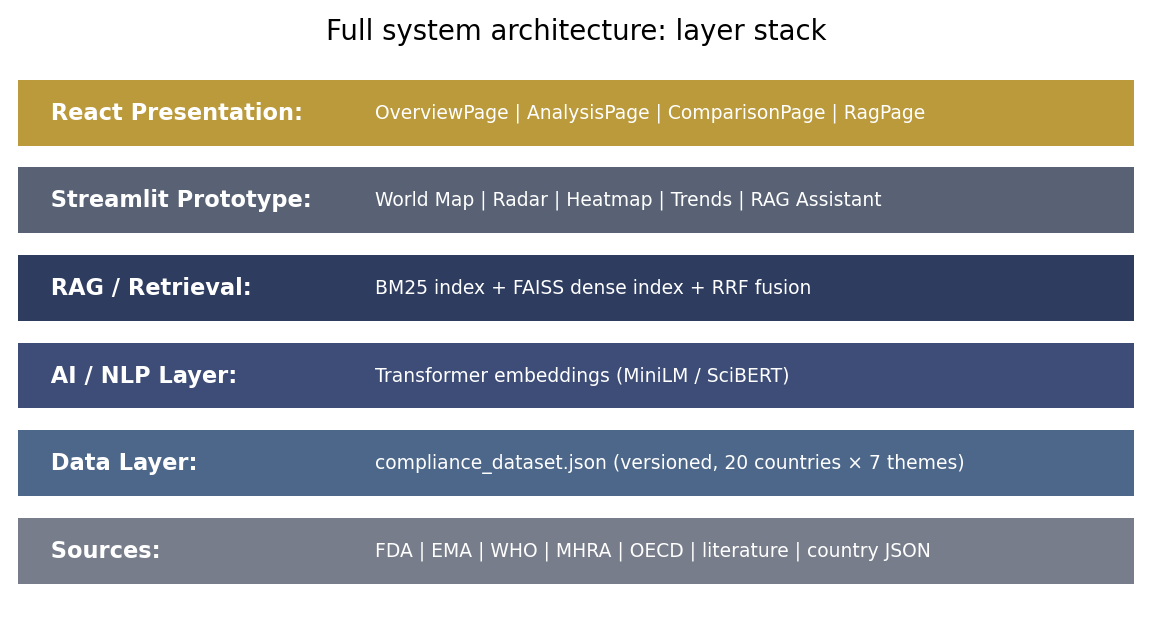
\includegraphics[width=0.82\textwidth]{figures/fig_dashboard_architecture.png}
\caption{Full dashboard architecture: six-layer stack from primary regulatory sources
  (bottom) to React and Streamlit presentation layers (top). Source: author.}
\label{fig:dash-arch}
\end{figure}

\subsection{Streamlit Prototype: Implementation Details}
\label{sec:dash-streamlit}

The Streamlit application loads the compliance dataset at startup and constructs a
Pandas DataFrame for tabular operations:

\begin{lstlisting}[caption={Streamlit data loading and sidebar filter logic},label={lst:streamlit},language=Python]
import streamlit as st
import pandas as pd, json, plotly.express as px

@st.cache_data
def load_data(path="data/compliance_dataset.json"):
    raw = json.loads(open(path).read())
    rows = []
    for c in raw["countries"]:
        row = {
            "country": c["country"],
            "region": c["region"],
            "maturity": c["maturity_level"],
            **c["themes_scores"]
        }
        rows.append(row)
    return pd.DataFrame(rows)

df = load_data()

# Sidebar filters (region, maturity, minimum theme threshold)
regions = st.sidebar.multiselect("Region", df.region.unique())
maturities = st.sidebar.multiselect("Maturity", df.maturity.unique())
min_score = st.sidebar.slider("Min composite score", 1.0, 10.0, 1.0)

# Apply filters
filtered = df.copy()
if regions:    filtered = filtered[filtered.region.isin(regions)]
if maturities: filtered = filtered[filtered.maturity.isin(maturities)]
THEME_KEYS = ["data_privacy","clinical_validation","approval_process",
              "transparency","ethics","post_market","liability"]
filtered["composite"] = filtered[THEME_KEYS].mean(axis=1)
filtered = filtered[filtered.composite >= min_score]
\end{lstlisting}

The six primary views are implemented as separate Streamlit tabs:

\begin{enumerate}[noitemsep]
  \item \textbf{World Map:} \texttt{px.choropleth} over ISO codes, coloured by
        composite $S_c$ or selected theme;
  \item \textbf{Country Comparison:} multi-select bar chart + radar via
        \texttt{plotly.graph\_objects.Scatterpolar};
  \item \textbf{Theme Analysis:} \texttt{px.imshow} heatmap of regional means plus
        gap charts $G_c^{\text{priv-liab}}$;
  \item \textbf{Global Trends:} trend cards rendered from
        \texttt{global\_trends} JSON array;
  \item \textbf{Country Details:} accordion narrative for any selected jurisdiction;
  \item \textbf{RAG Assistant:} text input $\to$ \texttt{hybrid\_retrieve} $\to$
        prompt injection $\to$ streamed LLM response with cited passages.
\end{enumerate}

\subsection{React Presentation Layer: Implementation Details}
\label{sec:dash-react}

\subsubsection{Component Hierarchy}

\begin{figure}[htbp]
\centering
\begin{tikzpicture}[
  comp/.style={draw=aivNavy!60, fill=aivBox, rounded corners=3pt,
               font=\scriptsize, minimum width=2.4cm, minimum height=0.65cm,
               align=center},
  page/.style={draw=aivNavy, fill=aivNavy!12, rounded corners=4pt,
               font=\small\bfseries, minimum width=2.8cm, minimum height=0.85cm,
               align=center},
  arr/.style={-{Latex[length=1.8mm]}, thin, aivNavy!70}
]
\node[page] (App) at (5.5, 4.5) {App};
\node[comp] (Ctx)  at (5.5, 3.4) {DashboardContext};
\node[page] (OV)   at (0.8, 2.0) {OverviewPage};
\node[page] (AN)   at (3.0, 2.0) {AnalysisPage};
\node[page] (CM)   at (5.2, 2.0) {ComparisonPage};
\node[page] (TR)   at (7.4, 2.0) {TrendsPage};
\node[page] (RG)   at (9.6, 2.0) {RagPage};
\node[comp] (MR)   at (0.8, 0.8) {MetricsRow};
\node[comp] (WM)   at (2.4, 0.8) {WorldMapTab};
\node[comp] (VT)   at (4.0, 0.8) {VisualTile};
\node[comp] (SI)   at (5.5, 0.8) {Sidebar +\\Slicers};
\node[comp] (RA)   at (7.5, 0.8) {RAGAssistant};
\draw[arr] (App) -- (Ctx);
\foreach \p in {OV,AN,CM,TR,RG}
  \draw[arr] (Ctx) -- (\p);
\draw[arr] (OV) -- (MR);
\draw[arr] (OV.south) -- (WM.north);
\draw[arr] (AN) -- (VT);
\draw[arr] (CM) -- (SI);
\draw[arr] (RG) -- (RA);
\end{tikzpicture}
\caption{React component hierarchy for the presentation dashboard. Source: author.}
\label{fig:react-tree}
\end{figure}

\subsubsection{Data Loading and State Management}

The \texttt{DashboardContext} loads \texttt{compliance\_dataset.json} from the
\texttt{public/} folder at initialisation, constructs typed arrays, and exposes
filtered slices via React context:

\begin{lstlisting}[caption={DashboardContext data loading (TypeScript excerpt)},label={lst:ctx},language=Python]
// src/context/DashboardContext.tsx
export const DashboardProvider: React.FC = ({ children }) => {
  const [data, setData] = useState<ComplianceDataset | null>(null);
  const [filters, setFilters] = useState<FilterState>(defaultFilters);

  useEffect(() => {
    fetch("/data/compliance_dataset.json")
      .then(r => r.json())
      .then(setData);
  }, []);

  const filtered = useMemo(() =>
    applyFilters(data?.countries ?? [], filters),
    [data, filters]
  );

  return (
    <DashboardCtx.Provider value={{ data, filtered, filters, setFilters }}>
      {children}
    </DashboardCtx.Provider>
  );
};
\end{lstlisting}

\subsubsection{Chart Implementations}

Recharts declarative API renders compliance charts with accessible colour palettes:

\begin{lstlisting}[caption={Radar chart for country theme comparison (Recharts)},label={lst:radar},language=Python]
// AnalysisPage.tsx -- radar comparison
<RadarChart data={radarData} width={400} height={340}>
  <PolarGrid stroke="#e2e8f0" />
  <PolarAngleAxis dataKey="theme" tick={{ fontSize: 11 }} />
  <PolarRadiusAxis domain={[0, 10]} tick={{ fontSize: 9 }} />
  {selected.map((country, i) => (
    <Radar key={country} name={country}
      dataKey={country}
      stroke={PALETTE[i % PALETTE.length]}
      fill={PALETTE[i % PALETTE.length]}
      fillOpacity={0.15}
    />
  ))}
  <Legend />
</RadarChart>
\end{lstlisting}

\subsection{RAG Assistant Frontend Integration}
\label{sec:dash-rag-frontend}

The \texttt{RagPage} component connects the React UI to the offline retriever via a
TypeScript wrapper (\texttt{src/lib/rag.ts}). The user experience is:

\begin{enumerate}[noitemsep]
  \item User types a compliance question in the query input field;
  \item The client calls \texttt{ragQuery(question, topK=6)};
  \item Retrieved passages are shown as expandable source cards with jurisdiction
        and theme tags;
  \item The grounded answer is streamed into a markdown-rendered response panel;
  \item Each sentence citation \texttt{[n]} links to the corresponding source card
        below, enabling immediate evidence inspection.
\end{enumerate}

A prominent disclaimer banner in the RAG Assistant panel reminds users that outputs
are research-grade information retrieval, not legal advice and not a substitute for
qualified regulatory counsel.

\subsection{Performance Optimisation}
\label{sec:dash-perf}

\begin{itemize}[noitemsep]
  \item \textbf{JSON caching:} \texttt{@st.cache\_data} in Streamlit; \texttt{useMemo}
        in React prevent redundant data reprocessing;
  \item \textbf{CSV export:} filtered DataFrame exported on demand rather than
        pre-computed, keeping bundle size minimal;
  \item \textbf{Offline FAISS:} flat L2 index over $\approx$3000 chunks completes a
        query in $<$15\,ms on a laptop CPU, well within interactive response budget;
  \item \textbf{Code splitting:} Vite tree-shakes unused Recharts components to keep
        the React bundle below 250\,kB gzipped.
\end{itemize}

\subsection{Testing and Quality Assurance}
\label{sec:dash-test}

The QA process covers three levels:

\begin{enumerate}[noitemsep]
  \item \textbf{Schema validation:} a Python script checks all required JSON keys,
        score ranges $[1,10]$, ISO code formats, and non-null narrative fields for
        Advanced jurisdictions;
  \item \textbf{Retrieval smoke tests:} five canonical compliance queries are run
        against the BM25 index and checked for non-empty top-3 results;
  \item \textbf{Dashboard walkthroughs:} three task-based scenarios---compare EU and
        US; identify the three lowest liability scores; run a RAG query on GDPR health
        data---are executed manually before each dataset version release.
\end{enumerate}

% -------------------------------------------------------------------------------
\section{System Integration and End-to-End Validation}
\label{sec:integration}
% -------------------------------------------------------------------------------

\subsection{Component Interface Specification}
\label{sec:interfaces}

All components communicate through a single versioned JSON contract. The schema
version field (\texttt{metadata.version}) is incremented whenever score cells, theme
definitions, or narrative fields change, ensuring that the React app, Streamlit app,
LaTeX report, and RAG corpus index remain synchronized.

\begin{equation}
\label{eq:version}
\texttt{JSON v}n \;\longrightarrow\;
\begin{cases}
\texttt{generate\_figures.py} & \text{(matplotlib figures)} \\
\texttt{streamlit run app.py} & \text{(Streamlit prototype)} \\
\texttt{npm run build} & \text{(React bundle)} \\
\texttt{pdflatex main.tex} & \text{(PDF report)}
\end{cases}
\end{equation}

\subsection{Reproducibility Runbook}
\label{sec:runbook-full}

Table~\ref{tab:runbook} specifies the complete reproduction sequence for an
independent examiner.

\begin{table}[htbp]
\centering
\caption{Complete reproduction runbook (clean environment)}
\label{tab:runbook}
\begin{tabular}{@{}clp{6.2cm}@{}}
\toprule
\textbf{Step} & \textbf{Command} & \textbf{Expected outcome} \\
\midrule
1 & \texttt{git clone \ldots} & Repository cloned \\
2 & \texttt{pip install -r requirements.txt} & Python dependencies installed \\
3 & \texttt{python generate\_figures.py} & All 13 figures written to \texttt{figures/} \\
4 & \texttt{streamlit run app.py} & Dashboard live at \texttt{localhost:8501} \\
5 & \texttt{cd web \&\& npm install \&\& npm run dev} & React app at \texttt{localhost:5173} \\
6 & \texttt{pdflatex main.tex} $\times$2 & PDF compiled, figures embedded \\
7 & \texttt{biber main; pdflatex main.tex} $\times$2 & Bibliography resolved \\
\bottomrule
\end{tabular}
\end{table}

\subsection{Chapter Summary}
\label{sec:techimpl-summary}

This chapter has specified the complete technical implementation of two core system
components: the AI techniques pipeline (transformer embeddings, ordinal scoring model,
use-case readiness model with disclosed theme weights, and the NLP classification
roadmap); and the interactive dashboard (Streamlit prototype, React presentation layer,
RAG Assistant frontend integration, performance optimisation, and QA protocol). The
RAG module---including corpus design, BM25+dense indexing, Reciprocal Rank Fusion,
prompt engineering, HITL integration, and evaluation---is fully documented in
Chapter~\ref{ch:rag}. Chapter~\ref{ch:results} now presents the empirical findings
produced by the complete platform.
